\documentclass[a4paper]{article}

\usepackage{geometry}
\usepackage{amsmath}
\usepackage{fontspec}
\usepackage{graphicx}
\usepackage{minted}

\usepackage{polyglossia}
\setmainlanguage[variant=american]{english}

\usepackage{hyperref}
\usepackage{subcaption}

\title{INF4300 -- Mandatory project -- Part 1}
\author{Bjørn Rustad}
\date{\today}

\begin{document}

\maketitle

\section{Analyzing the textures}

The textures to be analyzed are shown in Figure \ref{fig:raw_mosaic}. 

\begin{figure}
    \centering
    \begin{subfigure}[b]{0.40\textwidth}
        \centering
        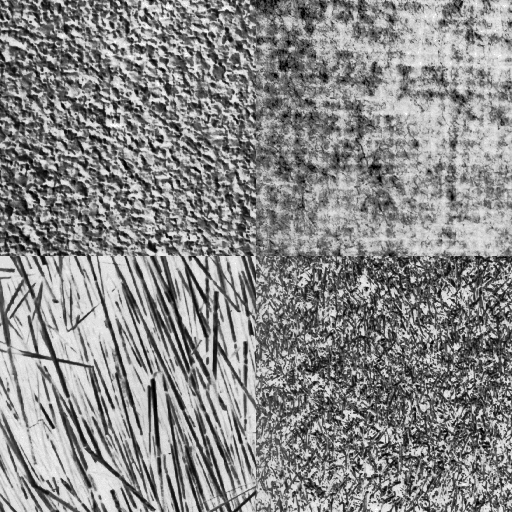
\includegraphics[width=\textwidth]{mosaic1.png}
        \caption{%
            Mosaic 1.
        }
    \end{subfigure}
    ~
    \begin{subfigure}[b]{0.40\textwidth}
        \centering
        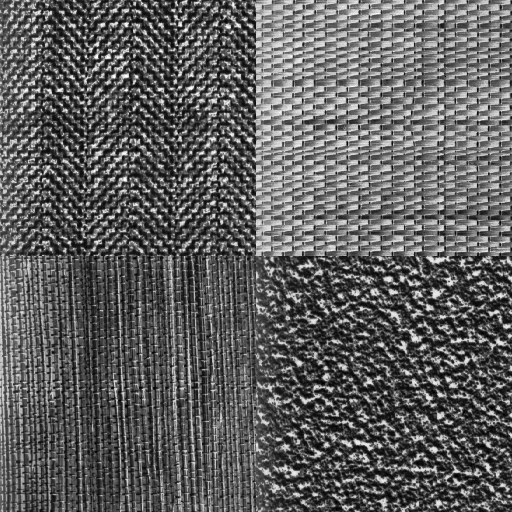
\includegraphics[width=\textwidth]{mosaic2.png}
        \caption{%
            Mosaic 2.
        }
    \end{subfigure}
    \caption{%
        Initial unprocessed mosaic images.
    }
    \label{fig:raw_mosaic}
\end{figure}

\subsection{Mosaic 1}

We start by looking at mosaic 1, which shows in the upper left corner an
relief-like texture with high contrast, no very strong directional
dependence, and a texel size of around 20x20 pixels. In the upper right
we see a more grid-like texture, where the grid is filled with hair-like
structures with varying intensity. I estimate the texel size to be in
the order of 20x20 pixels also here, but a difficulty is the varying
intensity in the texture. In the bottom left we see a very
different texture made of ``sticks'' laying mostly in the same direction,
and with quite high contrast. The texel size is harder to estimate as
some parts are more sparse on ``sticks'' than others, but
it is larger than in the other textures, about 40x40. In the bottom
right we have a very fine texture with no apparent direction, a smaller
texel size it has a higher frequency than the other textures.

\subsection{Mosaic 2}

Now in mosaic 2 we have in the upper left a fabric-like regular
texture. The texture direction varies, but in the vertical and
horizontal direction the texture appears pretty uniform. Ignoring the
direction changes it has a
small texel size of about 20x20 or less. The upper right texture is a very
homogenous braid-like texture with slightly larger texel size and a
uniform texture direction. The variance in grey level seems smaller than
the other textures. In the bottom left we have a very dark,
homogenous, bamboo-like texture with a uniform texture direction and a
texel size of about 20x20. Finally, in the bottom right we have a
homogenous but irregular texture of high contrast and no direction. It
also has a texel size of about 20x20.

\section{Visualizing the GLCM matrices}

Before analyzing the images, I perform a simple histogram equalization.
It visually seems like it enhances the contrast, and also removes some
of the spatially large variations in the background intensity. It will
also help us make more use of all the different levels in the GLCM
analysis.

Then we experiment with some different values for the GLCM matrices, and
visualize them for each of the different eight textures. Most of their
textures seem to have most of their information content in high contrast
changes, so we start with quite a low number of levels: $G = 6$. We
use symmetric GLCM, but not isotropic, since some of the textures are
directional, while others are not, so this might help us segment them.

As mentioned in the analysis, most of the textures are either
non-directional, or are quite uniform in both the vertical and
horizontal directions, so we start by trying $(dx, dy) = \{(3, 0), (0,
3)\}$.

The results for $(dx, dy) = (3, 0)$ are shown in Figure
\ref{fig:glcm6_3_0}. We see already that the upper two, and bottom left
textures of both mosaics are kind of discernible, while the bottom right
GLCM matrix is kind of similar to the upper left matrix in both mosaics.
Looking back at the mosaics, this is not so strange.

\begin{figure}
    \centering
    \begin{subfigure}[b]{0.40\textwidth}
        \centering
        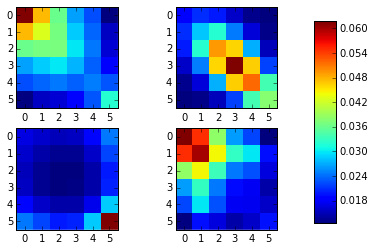
\includegraphics[width=\textwidth]{m1_3_0.png}
        \caption{%
            Mosaic 1.
        }
    \end{subfigure}
    ~
    \begin{subfigure}[b]{0.40\textwidth}
        \centering
        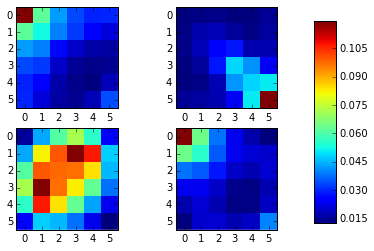
\includegraphics[width=\textwidth]{m2_3_0.png}
        \caption{%
            Mosaic 2.
        }
    \end{subfigure}
    \caption{%
        Six levels ($G = 6$), and $(dx, dy) = (3, 0)$.
    }
    \label{fig:glcm6_3_0}
\end{figure}

Although I do not expect very different results, for completeness we try
$(dx, dy) = (0, 3)$ in Figure \ref{fig:glcm6_0_3}.

\begin{figure}
    \centering
    \begin{subfigure}[b]{0.40\textwidth}
        \centering
        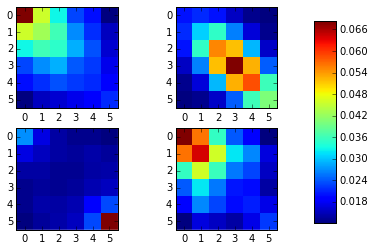
\includegraphics[width=\textwidth]{m1_0_3.png}
        \caption{%
            Mosaic 1.
        }
    \end{subfigure}
    ~
    \begin{subfigure}[b]{0.40\textwidth}
        \centering
        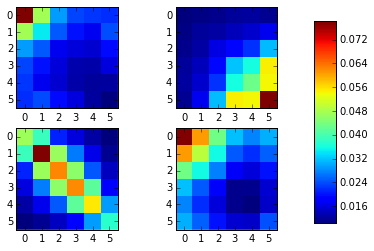
\includegraphics[width=\textwidth]{m2_0_3.png}
        \caption{%
            Mosaic 2.
        }
    \end{subfigure}
    \caption{%
        Six levels ($G = 6$), and $(dx, dy) = (0, 3)$.
    }
    \label{fig:glcm6_0_3}
\end{figure}

This is when I realize the values 0 and 3 for $dx$ and $dy$ are maybe
too small, and will be more affected by noise and small ``random''
variations than the actual texture appearance itself. Thus we try $(dx,
dy) = (10, 0)$, and to possibly increase the ``resolution'' GLCM matrix,
we increase the number of levels $G = 10$. Figure~\ref{fig:glcm10_10_0}
shows the resulting matrices.

\begin{figure}
    \centering
    \begin{subfigure}[b]{0.40\textwidth}
        \centering
        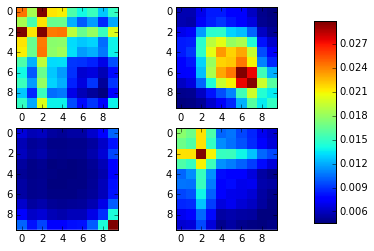
\includegraphics[width=\textwidth]{m1_10_0.png}
        \caption{%
            Mosaic 1.
        }
    \end{subfigure}
    ~
    \begin{subfigure}[b]{0.40\textwidth}
        \centering
        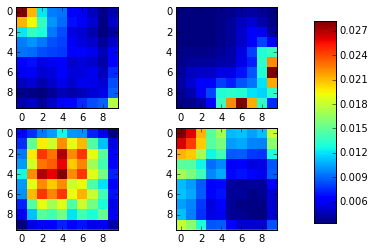
\includegraphics[width=\textwidth]{m2_10_0.png}
        \caption{%
            Mosaic 2.
        }
    \end{subfigure}
    \caption{%
        Ten levels ($G = 10$), and $(dx, dy) = (10, 0)$.
    }
    \label{fig:glcm10_10_0}
\end{figure}

As before, the top left and bottom right matrices are still a bit
similar, but now a bit more discernible if one considers the «inertia»
weighting, i.e.\ how much weight is concentrated far from the diagonal
axis.

From the three GLCM features listed in the assignment, I would think
cluster shade is the one giving the most valuable information looking at
these GLCM matrices. The cluster shade weights the matrix with a
gradient going from negative values in the upper left corner to positive
values in the lower right corner, and thus measures how the matrix is
balanced along the diagonal. Looking at the different GLCM matrices,
this could help us differentiate between all of the four textures in
each mosaic except maybe the top left from the bottom right. As the top
left square only touches the bottom right square in the middle, a
sofisticated enough segmentation step should manage to separate them
even if they have feature values in the same range.

To separate the top left from the bottom right textures, in both
mosaics, it seems like GLCM inertia would be a better feature, as the
distribution around the diagonal is a bit different, especially for the
parameters $G = 10$, $(dx, dy) = (10, 0)$ in Figure
\ref{fig:glcm10_10_0}.

\section{GLCM on local windows}

To be able to segment the textures, we calculate the GLCM matrix and
from it the GLCM features on a window that we slide over the two
mosaics. We choose odd window sizes so that the windows are centered
around a pixel, and thus we get a feature value in each pixel position
except for a border around the edge of the image. 

We calculate the GLCM homogeneity, intertia, and cluster shade features,
and they are implemented in Appendix \ref{app:code}.

For the GLCM matrices with $G = 6$ and $(dx, dy) = \{(3, 0), (0, 3)\}$,
shown in Figure \ref{fig:glcm6_3_0} and \ref{fig:glcm6_0_3} we select a
feature size of 31-by-31. The initial analysis indicated that this is a
bit more than the size of most of the texels. For the GLCM with $G = 10$ and
$(dx, dy) = (10, 0)$ visualized in Figure \ref{fig:glcm10_10_0}, we
select a larger window size of 41-by-41, as this GLCM was intended to be
better at separating the very similar textures.

As my Python implementation of the GLCM calculation apparently was not
super efficient, I use a stride of 5 pixels in each direction, giving a
speedup of about 25 times. As this is much less than our window size of
31 and 41, I do not think this affects the results a lot, except for a
larger uncertainty around the borders between the textures.

\subsection{Homogeneity}

\begin{figure}
    \centering
    \begin{subfigure}[b]{0.30\textwidth}
        \centering
        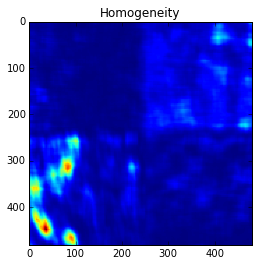
\includegraphics[width=\textwidth]{hom11.png}
        \caption{%
            $H_{1,1}$
        }
        \label{fig:h11}
    \end{subfigure}
    ~
    \begin{subfigure}[b]{0.30\textwidth}
        \centering
        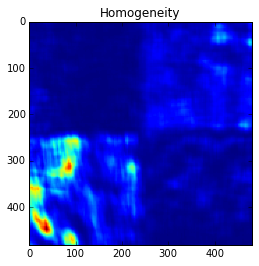
\includegraphics[width=\textwidth]{hom21.png}
        \caption{%
            $H_{2,1}$
        }
        \label{fig:h21}
    \end{subfigure}
    ~
    \begin{subfigure}[b]{0.30\textwidth}
        \centering
        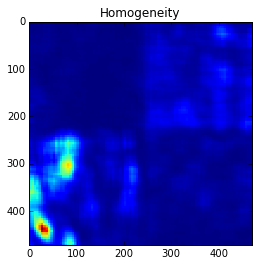
\includegraphics[width=\textwidth]{hom31.png}
        \caption{%
            $H_{3,1}$
        }
        \label{fig:h31}
    \end{subfigure}
    \\
    \begin{subfigure}[b]{0.30\textwidth}
        \centering
        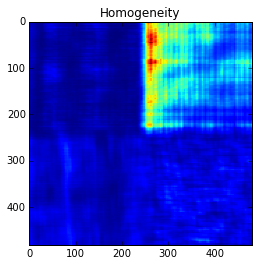
\includegraphics[width=\textwidth]{hom12.png}
        \caption{%
            $H_{1,2}$, \\
            $G=6$, $(dx, dy)=(3,0)$
        }
        \label{fig:h12}
    \end{subfigure}
    ~
    \begin{subfigure}[b]{0.30\textwidth}
        \centering
        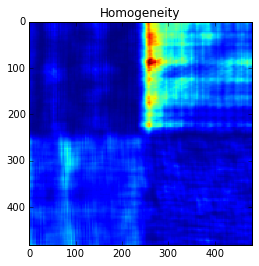
\includegraphics[width=\textwidth]{hom22.png}
        \caption{%
            $H_{2,2}$, \\
            $G=6$, $(dx, dy)=(0,3)$
        }
        \label{fig:h22}
    \end{subfigure}
    ~
    \begin{subfigure}[b]{0.30\textwidth}
        \centering
        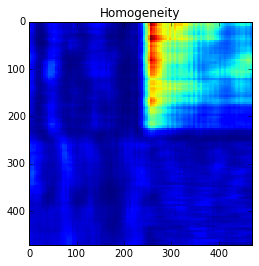
\includegraphics[width=\textwidth]{hom32.png}
        \caption{%
            $H_{3,2}$, \\
            $G=10$, $(dx, dy)=(10,0)$
        }
        \label{fig:h32}
    \end{subfigure}

    \caption{%
        Homogeneity feature shown for mosaic 1 on top and mosaic 2 on
        the bottom, with the different selected GLCM parameters from
        left to right.
    }
    \label{fig:hom}
\end{figure}

The homogeneity (or angular second moment) feature is shown in Figure
\ref{fig:hom}, for all the parameters selected previously. It seems like
this homogeneity feature could be used to attempt to segment out the top
right texture of mosaic 2. In hindsight we could maybe have chosen the
GLCM parameters $dx$ and $dy$ specifically with homogeneity in mind to
segment out the very homogenous top right and bottom left textures of
mosaic 2.

\subsection{Inertia}

\begin{figure}
    \centering
    \begin{subfigure}[b]{0.30\textwidth}
        \centering
        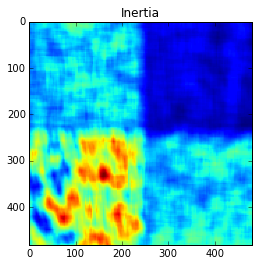
\includegraphics[width=\textwidth]{inertia11.png}
        \caption{%
            $I_{1,1}$
        }
        \label{fig:i11}
    \end{subfigure}
    ~
    \begin{subfigure}[b]{0.30\textwidth}
        \centering
        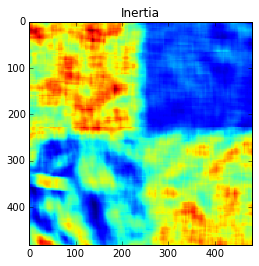
\includegraphics[width=\textwidth]{inertia21.png}
        \caption{%
            $I_{2,1}$
        }
        \label{fig:i21}
    \end{subfigure}
    ~
    \begin{subfigure}[b]{0.30\textwidth}
        \centering
        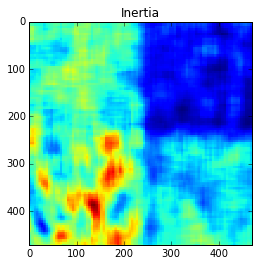
\includegraphics[width=\textwidth]{inertia31.png}
        \caption{%
            $I_{3,1}$
        }
        \label{fig:i31}
    \end{subfigure}
    \\
    \begin{subfigure}[b]{0.30\textwidth}
        \centering
        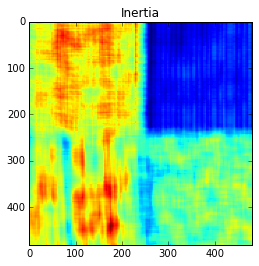
\includegraphics[width=\textwidth]{inertia12.png}
        \caption{%
            $I_{1,2}$, \\
            $G=6$, $(dx, dy)=(3,0)$
        }
        \label{fig:i12}
    \end{subfigure}
    ~
    \begin{subfigure}[b]{0.30\textwidth}
        \centering
        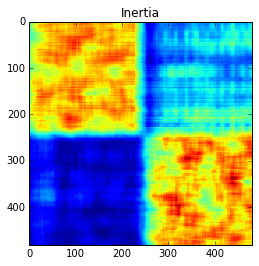
\includegraphics[width=\textwidth]{inertia22.png}
        \caption{%
            $I_{2,2}$, \\
            $G=6$, $(dx, dy)=(0,3)$
        }
        \label{fig:i22}
    \end{subfigure}
    ~
    \begin{subfigure}[b]{0.30\textwidth}
        \centering
        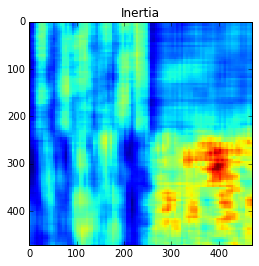
\includegraphics[width=\textwidth]{inertia32.png}
        \caption{%
            $I_{3,2}$, \\
            $G=10$, $(dx, dy)=(10,0)$
        }
        \label{fig:i32}
    \end{subfigure}

    \caption{%
        Inertia feature shown for mosaic 1 on top and mosaic 2 on
        the bottom, with the different selected GLCM parameters from
        left to right.
    }
    \label{fig:inertia}
\end{figure}

The inertia feature is shown in Figure \ref{fig:inertia}. It worked
well, maybe even better than expected. It seems like it can be used to
successfully segment out the top right texture of mosaic 1, and also the
top right and bottom left textures of mosaic 2. As opposed to the
homogeneity measure, it performs very differently for the different GLCM
parameters, which is nice.

It seems like the bottom left texture of mosaic 1, which is a difficult
texture with a large texel size, can at least be partially segmented out
using the inertia feature.

\subsection{Cluster shade}

\begin{figure}
    \centering
    \begin{subfigure}[b]{0.30\textwidth}
        \centering
        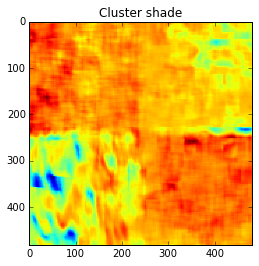
\includegraphics[width=\textwidth]{cls11.png}
        \caption{%
            $C_{1,1}$
        }
        \label{fig:c11}
    \end{subfigure}
    ~
    \begin{subfigure}[b]{0.30\textwidth}
        \centering
        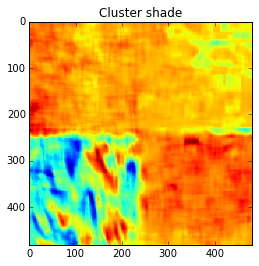
\includegraphics[width=\textwidth]{cls21.png}
        \caption{%
            $C_{2,1}$
        }
        \label{fig:c21}
    \end{subfigure}
    ~
    \begin{subfigure}[b]{0.30\textwidth}
        \centering
        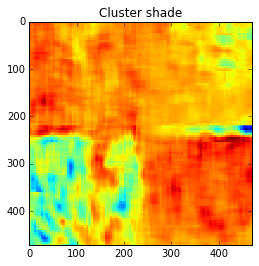
\includegraphics[width=\textwidth]{cls31.png}
        \caption{%
            $C_{3,1}$
        }
        \label{fig:c31}
    \end{subfigure}
    \\
    \begin{subfigure}[b]{0.30\textwidth}
        \centering
        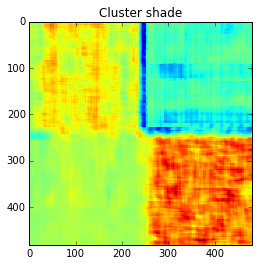
\includegraphics[width=\textwidth]{cls12.png}
        \caption{%
            $C_{1,2}$, \\
            $G=6$, $(dx, dy)=(3,0)$
        }
        \label{fig:c12}
    \end{subfigure}
    ~
    \begin{subfigure}[b]{0.30\textwidth}
        \centering
        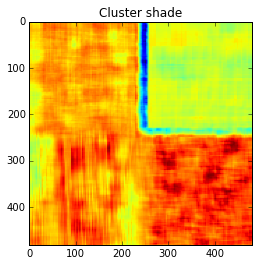
\includegraphics[width=\textwidth]{cls22.png}
        \caption{%
            $C_{2,2}$, \\
            $G=6$, $(dx, dy)=(0,3)$
        }
        \label{fig:c22}
    \end{subfigure}
    ~
    \begin{subfigure}[b]{0.30\textwidth}
        \centering
        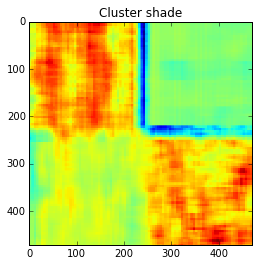
\includegraphics[width=\textwidth]{cls32.png}
        \caption{%
            $C_{3,2}$, \\
            $G=10$, $(dx, dy)=(10,0)$
        }
        \label{fig:c32}
    \end{subfigure}

    \caption{%
        Cluster shade feature shown for mosaic 1 on top and mosaic 2 on
        the bottom, with the different selected GLCM parameters from
        left to right.
    }
    \label{fig:cls}
\end{figure}

The cluster shade feature is shown in Figure \ref{fig:cls}. It did not
seem to work as well as hoped in the analysis. In mosaic 1 it seems like
we could manage to extract at least a partial segmentation of the bottom
left texture. Apart from that the cluster shade dissapointed a bit as a
feature for mosaic 1. Looking back at the matrices in Figure
\ref{fig:glcm6_3_0}, it seemed like we should also have been able to see
a difference between the top left and the top right textures.

For mosaic 2, the cluster shade feature works better. We should be able
to segment out both the top right and also the bottom right texture
quite well.

\section{Segmenting by thresholding}

As briefly discussed in the previous section, we will here try to
segment out the different textures by thresholding the feature images.
In overview it seems like we did a better job with the features for
segmenting mosaic 2.

We would also need some kind of method to remove small noise inside and
outside the segmented region, which should be based on some prior belief
that our regions are somewhat large and connected.

Because of a window size of 31 and 41, and in addition a stride of 5, we
see that we are not really able to touch the center with all the
segmented regions, although some of them look quite OK in that regard.

\subsection{Mosaic 1}

\begin{figure}
    \centering
    \begin{subfigure}[b]{0.30\textwidth}
        \centering
        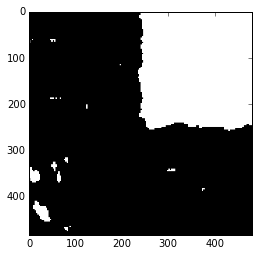
\includegraphics[width=\textwidth]{segm_1_i11.png}
        \caption{%
            $I_{1,1} < 3$
        }
    \end{subfigure}
    ~
    \begin{subfigure}[b]{0.30\textwidth}
        \centering
        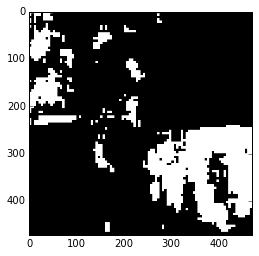
\includegraphics[width=\textwidth]{segm_1_c31.png}
        \caption{%
            $C_{3,1} > 15$
        }
    \end{subfigure}
    ~
    \begin{subfigure}[b]{0.30\textwidth}
        \centering
        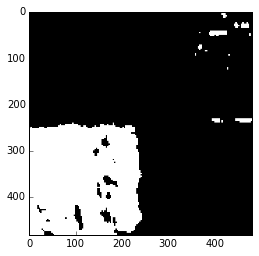
\includegraphics[width=\textwidth]{segm_1_c21_i11.png}
        \caption{%
            $C_{2,1} < -10 \cup I_{1,1} > 7$
        }
    \end{subfigure}
    \caption{%
        Thresholding applied to segment out the different textures of
        mosaic 1.
    }
    \label{fig:m1_segm}
\end{figure}

Starting with mosaic 1 we experiment to find good thresholds on the
different features. The results can be seen in Figure \ref{fig:m1_segm}.
We manage to segment out the top right texture quite well, with little
noise inside and outside the segmented region.

The bottom right is more difficult, and the threshold given is a
compromise between noise inside and outside the region, but the size of
the size of the noise seems to big to tackle with simple methods. Better
GLCM parameters and/or other features are probably needed to properly
segment this region. In hindsight, the choice of $dx$ and $dy$ only in
$\{0, 3, 10\}$ was probably a bit too limiting, as for example the
bottom right and top left texture differ a little bit in the frequency
of the smallest variations.

The segmentation of the bottom left looks OK with noise of small spatial
size, both inside and outside the region.

To extract the top left patch we can subtract the three shown images
from a white image, which would of course include some noise from the
poorly segmented bottom right region.

\subsection{Mosaic 2}

\begin{figure}
    \centering
    \begin{subfigure}[b]{0.23\textwidth}
        \centering
        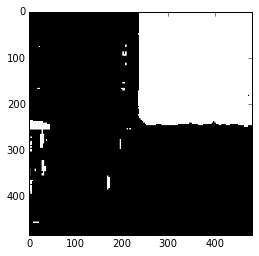
\includegraphics[width=\textwidth]{segm_2_c12_low.png}
        \caption{%
            $C_{1,2} < -1.5$
        }
    \end{subfigure}
    ~
    \begin{subfigure}[b]{0.23\textwidth}
        \centering
        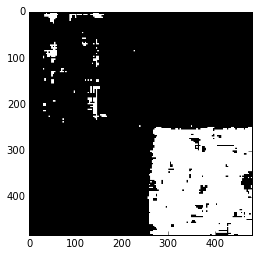
\includegraphics[width=\textwidth]{segm_2_c12_hi.png}
        \caption{%
            $C_{1,2} > 7$
        }
    \end{subfigure}
    ~
    \begin{subfigure}[b]{0.23\textwidth}
        \centering
        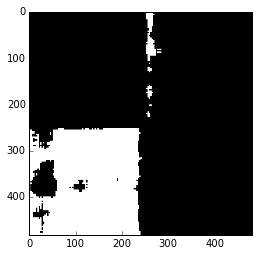
\includegraphics[width=\textwidth]{segm_2_i22_low.png}
        \caption{%
            $I_{2,2} < 2$
        }
    \end{subfigure}
    ~
    \begin{subfigure}[b]{0.23\textwidth}
        \centering
        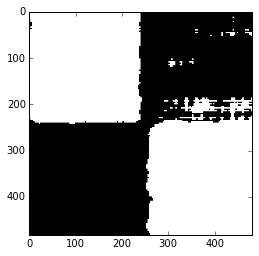
\includegraphics[width=\textwidth]{segm_2_i22_hi.png}
        \caption{%
            $I_{2,2} > 4$
        }
    \end{subfigure}
    \caption{%
        Thresholding applied to segment out the different textures of
        mosaic 2.
    }
    \label{fig:m2_segm}
\end{figure}
\appendix

The results of efforts to segment the different parts of mosaic 2 can be
seen in Figure~\ref{fig:m2_segm}. The results are in general better than
for mosaic 1. It seems like the combination of GLCM parameters and
features worked better here, which can also be because mosaic 2 appears
more uniform and regular.

Also for mosaic 2 does the top right texture segment well. The
segmentation of the bottom right is OK, except that it does not hit the
center, and contains some small sized noise. Segmenting the bottom left
texture using the inertia goes OK except for a big black hole to the
left, which is a bit bigger than we would have wanted, but maybe
finetuning the threshold could help.

Using the inertia also gives a good joint segmentation of the top left
and bottom right textures. Separating them could be done by some kind of
search for large connected components, or by subtracting the previous
segmentation of the bottom left texture.

Again, a segmentation of the top left texture can be obtained by a
combination of the other thresholded images.

\section{Code}
\label{app:code}

\subsection{GLCM calculation}
\inputminted{python}{../glcm.py}

\subsection{Feature experimentation}
\inputminted{python}{analysis.py}

\end{document}

